  
\documentclass[titlepage]{article}
\usepackage[utf8]{inputenc}
\usepackage{amsmath}
\usepackage{tcolorbox}
\usepackage{amssymb}
\usepackage{amsthm}
\usepackage{empheq}
\usepackage{xcolor}

\usepackage[utf8]{inputenc}
\usepackage{amsmath}
\usepackage{tcolorbox}
\usepackage{amssymb}
\usepackage{amsthm}
\usepackage{physics}
\usepackage{empheq}
\usepackage{xcolor}
\usepackage{float}
\usepackage{float}
\usepackage[
top    = 2.50cm,
bottom = 2.50cm,
left   = 2.75cm,
right  = 2.75cm]{geometry}
\usepackage{fancyhdr}
\pagestyle{fancy}
\lhead{Analysis 2}
\rhead{EPFL/Alp Ozen}

\newtheorem{remark}{Remark}[section]
\newtheorem{theorem}{Theorem}[section]
\newtheorem{prop}{[Proposition]}
\newtheorem{definition}{Definition}
\newtheorem{question}{Question}

\newcommand{\interior}[1]{%
  {\kern0pt#1}^{\mathrm{o}}%
}
\newcommand{\Rn}{\mathbb{R}^n}
\newcommand{\Rm}{\mathbb{R}^m}
\newcommand{\R}{\mathbb{R}}

\title{\textbf{Analysis 2 - Thomas Mountford}}
\author{Alp Ozen}
\date{Spring 2019}
\newtheorem{example}{Example}[section]
\newtheorem{axiom}{Axiom}
\newtheorem{cor}{Corollary}

\begin{document}

\maketitle
\tableofcontents
\clearpage


\section{Notions on \Rn}

\subsection{Introducing topological properties on \Rn}
Let's recall that $\Rn$ is a Euclidean vector space. We define a scalar product on $\Rn$ as follows:

\begin{definition}
\begin{equation*}
    < \cdot, \cdot > : \Rn \times \Rn \to \mathbb{R}
\end{equation*}


\begin{enumerate}
    \item $<x,x> \geq 0$
    \item $<x,y> = <y,x>$
    \item $<ax + by, z> = a<x,z> + b<y,z>$
\end{enumerate}

\end{definition}


A \textit{norm} is defined as function that maps some real vector space $E$ to $\mathbb{R}$ and satisfies:

\begin{align*}
    1) \ |x| \geq 0 \ \forall x \in E, \ |x| = 0 \iff x = 0\\
    2) \ |\lambda \cdot x| = |\lambda| \cdot |x| \\
    3) \ |x+y| \leq |x| + |y|
\end{align*}

In our intuitive understanding of $\Rn$ we are actually thinking about the Euclidian space $\Rn$ equipped with the Euclidian norm.

\begin{definition}\textbf{Euclidian norm}
$$|x|_{2} = \sqrt{<x,x>} = (\sum^{n}_{i}x^{2}_{k} )^{\frac{1}{2}} $$
\end{definition}

And from this naturally follows the definition of Euclidian distance:
\begin{definition}
$$d(x,y) = |x-y|$$
\end{definition}

We note that $d$ satisfies the same 3 properties as the norm. Thus, the couple \textbf{$(E,d)$} is called a metric space. 
\\

And now more definitions:

\begin{definition} \textbf{Open sets}
\begin{enumerate}
    \\
    
    \item \textbf{Open ball} $ B(a,r) := \{x \in \Rn : d(x,a) < r\}$
    \item \textbf{Open subset} Some subset $S \subset \Rn$ is open if $\forall x \in \Rn, \ \exists \epsilon > 0 \ B(x,\epsilon) \subset S$
    \item \textbf{Closed subset} Some $S$ is closed if $\Rn - S$ is open, note that the empty set and $\Rn$ are both open and closed. 
    \item \textbf{The interior and boundary of a set} $a$ is in the interior of $S$ if $\exists \epsilon > 0 \ B(a,\epsilon) \subset S$ and $b$ is in the boundary of a set $S$ if any $B(a, \epsilon)$ contains points from both $S$ and $\Rn - S$. The set of all interior points is denoted $\interior(S)$ and set of all boundary points is denoted $\partial S$
    \item \textbf{Closure of a set} $a$ is a closure of $S$ if for any $B(a,\epsilon)$ we have $B(a, \epsilon) \cap S \not = \emptyset$ 
\end{enumerate}

\end{definition}

\begin{definition}\textbf{Topology}

A Topology exists whenever the following are satisfied:

$$\text{For a given} \ M \subset \Rn \text{we define} \ O \subset P(M) $$
\begin{enumerate}
    \item $\emptyset \in O \ , M \in O $
    \item $U \in O, V \in O \rightarrow U \cap V \in O$
    \item $U_{\alpha} \in O \rightarrow \bigcup_{\alpha} U_{\alpha} \in O$
\end{enumerate}

\end{definition}


\begin{definition}\textbf{Closure of a set}
A point $a \in \Rn$ is a closure point of $S$ if for any $B(a,\epsilon)$ we have:
$$B(a,\epsilon) \cap S \not = \emptyset$$
The set of all closure points called the closure of $S$ is denoted $\bar{S}$ noting that this only holds in $\Rn$

$$\bar{S} = S \cup \partial S$$
\end{definition}

\begin{theorem}
Important results on closures and boundaries
\begin{align*}
    \interior{S} \subset S \subset \bar{S}\\
    \bar{S} = \interior{S} \cup \partial S\\
    S \ \text{is open iff} \ S = \interior{S}\\
    S \ \text{is closed iff} \ S = \bar{S}\\
\end{align*}
    
\end{theorem}

\begin{definition} \textbf{Sequence in \Rn}
\\

$f : \mathbb{N} \to \Rn$ such that:
$$x_{k} = f(k) \in \Rn \forall k \in \mathbb{N}$$

\end{definition}


\begin{definition} \textbf{Convergence}
\\

The definition of convergence in $\Rn$ is very similar to its counterpart in $\mathbb{R}$. We say that $x_{k}$ converges to $x$ iff:

$$ \forall \epsilon > 0 \ \exists N_{\epsilon} \ \forall k \geq N_{\epsilon} \ d_{2}(x_{k},x}) < \epsilon$$
\end{definition}


\begin{definition} \textbf{Complete spaces aka. Banach spaces}
\\
A space is called complete if every Cauchy sequence in this space converges to a limit. Some example of complete spaces are $\mathbb{R}, \Rn$
\end{definition}

We restate the axioms of a \textbf{Norm} and of a \textbf{Metric}. The subtle difference between the two is that a norm can only be applied to some vector space whereas a metric is applicable to other spaces.
\begin{remark} \textbf{Axioms of norm and metric}
\\
\textbf{Norm:}
\begin{enumerate}
    \item $||x|| \geq 0$
    \item $ ||\lambda x|| = |\lambda| ||x||$
    \item $||x+y|| \leq ||x|| + ||y||$
\end{enumerate}
\end{remark}
\\

\textbf{Metric:}
\begin{enumerate}
    \item $d(x,y) \geq 0$
    \item $d(x,y) = d(y,x)$
    \item $d(x,y) \leq d(x,z) + d(z,y)$
\end{enumerate}

\subsection{Difficult problems and notes from week 2}
We note that any open set is equal to its interior. 

\begin{example}
Consider the set defined as $ T = \{(x,y) \in \mathbb{R}^{2} | 1 < x^{2} + 4y^{2} < 4 \}$
We observe the following about this set:

\begin{align*}
     \interior{T} = T \\
     \partial{T} = \{(x,y) \in \mathbb{R}^{2} | 1 = x^{2} + 4y^{2} \text{or} \ x^{2} + 4y^{2} = 4 \}
\end{align*}
\end{example}

\begin{remark}
Rather interestingly, the rational numbers are neither closed nor open because both the irrationals are dense as well as the rationals being dense which was proved in analysis 1. We have the following properties for $\mathbb{Q}$

$$ \partial \mathbb{Q} = \bar{\mathbb{Q}} = \R$$
\end{remark}

\begin{definition}
If $x_{k}$ is in a bounded closed set $D$ then $\exists$ a convergent subsequence with limit in $D$.
\end{definition}

\begin{definition} \textbf{Continuity open ball definition}
\\
$\forall a \in \Rn$ we have $\forall \epsilon > 0$ $\exists \delta > 0 $ such that $f(B(a,\delta)) \subset B(f(a), \epsilon)$
\end{definition}

\begin{definition} \textbf{Continuity open set definition}
\\
Let $f: \Rn \to \Rm$ Then $f$ is continuous on $\Rn$ iff. for all $ O \subset \Rm$ where $O$ is open, we have $f^{-1}(O)$ open in $\Rn$
\end{definition}

\begin{proof}
\\
\textbf{(only if part)}
Let $f$ be continuous, we want to show that whenever $O$ is open, $f^{-1}(O)$ is also open. Now take $f^{-1}(O)$. Let $p \in f^{-1}(O)$. Then $f(p) \in O$ Now we have that $O$ is open hence $\exists \epsilon > 0$ s.t. $B(f(p),\epsilon) \subset O$ Now because $f$ is continuous at $p$ we have that $\exists \delta > 0$ s.t. $\underbrace{f(B(p, \delta)) \subseteq B(f(p), \epsilon)}_{\text{applying open ball cont.}} \subseteq O$ This further shows that $B(p, \delta) \subseteq f^{-1}(O)$ which shows that $f$ is open in $S$.
\\

\textbf{(if part)}
Now suppose that for all open sets $O \in \Rm$ we have $f^{-1}(V)$ are open in $S$. To show that $f$ is continuous, we must show $f$ is continuous on all $p \in S$. Let $p \in S$ s.t. $y = f(p)$. Then $\forall \epsilon > 0$ $B(y,\epsilon)$ is open. By assumption then, $f^{-1}(B(f(p), \epsilon))$ is open in $S$. Now, $f(p) \in B(f(p), \epsilon)$ we have $p \in f^{-1}(B(f(p), \epsilon))$ is open in $S$, $\exists \delta > 0$ s.t. $B(p, \delta) \subseteq f^{-1}(B(f(p), \epsilon))$ and applying $f$ to both sides we get our result. 
\end{proof}

\subsection{More norms on \Rn}
Consider the non-usual norms $|x|_{1} := \sum |x|$ and $|x|_{\infty} = max |x_{k}|$. A super interesting result is that all norms on $\Rn$ are equivalent. 

\begin{definition}
Two norms $|\cdot|$ and $||\cdot||$ are \textbf{equivalent} if $\exists C_{1}, C_{2} > 0$ such that $\forall x \in E \ :$

$$C_{1}|x| \leq ||x|| \leq C_{2}|\cdot|$$
\end{definition}

\begin{theorem}
Any two norms on $\Rn$ are equivalent. 
\end{theorem}

We do not prove this theorem but consider the visual below for why it is true. 
\begin{figure}[H]
    \centering
    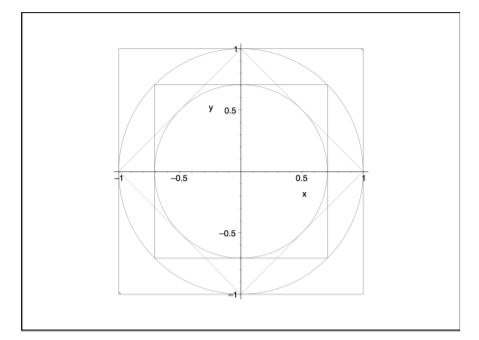
\includegraphics[scale = 0.4]{src/normEQ.JPG}
    \caption{Norm equivalence}
    \label{fig:my_label}
\end{figure}

\subsection{Curves in \Rn}
\begin{definition}\textbf{Curve}
A curve is a function $f: I \to \Rn$ denoted as:
$$f = \begin{bmatrix}
f_{1}\\
\vdots \\
f_{n}
\end{bmatrix}$$
\end{definition}

A good example of a curve is the speed of a particle in mechanics. It takes only one input $t$ and has a different function defined for each coordinate. Another example is the graph $G_{f} = \begin{bmatrix}
x\\
f(X)
\end{bmatrix}$ of any function from $I \to \mathbb{R^{2}}$
Another curve is a helix defined as:
\begin{definition}\textbf{Helix}
$$f(t) = \begin{bmatrix}
r\cos{t}\\
r\sin{t}\\
ct
\end{bmatrix}$$
\end{definition}

\begin{figure}[H]
    \centering
    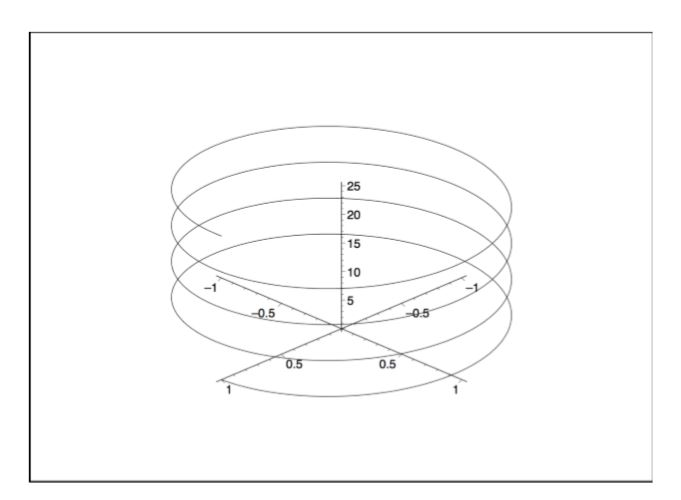
\includegraphics{src/helix.JPG}
    \caption{Helix}
    \label{fig:my_label}
\end{figure}


\begin{definition}\textbf{Arc-length of a curve}
Given a curve is rectifiable(each segment tends to 0 and sum of segments tend to $L>0$ we define
$$ L = \int_{b}^{a}|f^{\prime}(t)|_{2}dt$$
\end{definition}

Now the above formula is taught at high school level as:
$$ L = \int_{b}^{a}f^{\prime}\sqrt{1 + \frac{dx}{dy}^{2}} dx$$ which is simply the application of our definition to $\mathbb{R}^{2}$

\subsection{Real-valued functions in \Rn}

\begin{definition}\textbf{Real valued function}
$f: D \to \mathbb{R}$ such that $D \subset \Rn$
\end{definition}

The graph $G_{f}$ of a real valued function is the set $G_{f} = \{ \begin{bmatrix} x\\
f(x)
\end{bmatrix} | | x \in D\} \subset \mathbb{R}^{n+1}$

Hence where a curve is map from one dimension to $n$ dimensions, a real-valued function is a map from $n$ dimensions to 1 dimension. 



\subsection{Partial derivatives}

\begin{definition}
$f:\Rn \to \mathbb{R}$ is partially differentiable with respect to variable $x_{k}$ if:
$$\frac{\partial f}{\partial x_{k}}(a) = \lim \frac{f(a+he_{k}) - f(a)}{h}$$ exists. To calculate the partial derivative at $x_{k}$ we simply let all $x_{i}$ be constants. 
\end{definition}

\begin{definition}\textbf{Gradient}
The gradient of $f$ is defined as:

$$ \nabla f(x) = \begin{bmatrix}
\frac{\partial f}{\partial x_{1}}(a)\\
\vdots\\
\frac{\partial f}{\partial x_{n}}(a)
\end{bmatrix} = \sum_{k=1}^{n} D_{k}f(x)e_{k}$$

\end{definition}

\begin{example}
Let $f(x) = |x|_{2}$ Then we have that $\frac{\partial f}{\partial x_{k}}(a) = \frac{x_{k}}{r}$
\end{example}

Now we come to a more complicated example: 

\begin{example}
$$f(x,y) = \[ \begin{cases}  
      \frac{xy}{x^{2} + y^{2}} (x,y) \not = 0\\
      0 (x,y) = 0
   \end{cases}
\]$$

In this case, we have that although the partial derivative exists its existence does not imply continuity. The partial derivative itself must be continuous to imply continuity. 
\end{example}



\begin{definition}\textbf{Continuity in \Rn}
\\

We say that $f: \Rn \to \mathbb{R}$ is continuous at $a \in \Rn$ if $\forall \epsilon > 0 \ \exists \delta > 0$ such that $|x-a|_{2} < \delta \rightarrow |f(x) - f(a)|_{2} < \epsilon$
\end{definition}

The problem with the above definition is that we may approach say $(0,0)$ from infinite number of ways(easily seen considering a cartesian plane). This was not the case in $\mathbb{R^{1}}$ because we could approach 0 from the left or the right. Hence to prove that a limit exists by using cases is impossible, we need to instead use the epsilon-delta definition. 


\begin{definition}
We define $C^{1}(U)$ as the set of functions $f: U\subset \Rn \to R$ such that $f$ has $n$ partial derivatives each continuous. 
\end{definition}

\begin{definition}\textbf{Contour graphs}
When we are presented with a real-valued function of multiple variables, we may either represent it via its graph, that is map it to $\mathbb{R}^{m+1}$ or instead draw its contour lines that is we let the function equal some value $c \in \mathbb{R}$ and plot all the points in $\mathbb{R^{m}}$ that take this value.

\end{definition}

And now we define the total differential. 

\begin{definition}\textbf{Total differential}
$$dz = \frac{\partial z}{\partial x}dx + \frac{\partial z}{\partial y}dy$$
\end{definition}

Well when might the total differential ever be useful? Here's a simple example.

\begin{example}
Let's define $z = \sqrt{x^{2} + y^{2}}$ Now suppose we want to evaluate the function at $(x=3.92, y=4.01)$ Then we may simply evaluate the function at $(x=4, y=4)$ and using the total differential find the change in z and subtract it from our initial result. 
\end{example}

\begin{definition}\textbf{Bilinear form}
We may think of a bilinear form as a linear map that accepts 2 arguments instead of one and linearity holds for both arguments. 

$$B: V\cross V \to F$$
\begin{align*}
    B(v_{1}+v_{2},w) = B(v_{1},w) + B(v_{2},w)\\
    B(fv,w) = fB(v,w)\\
    B(v,w_{1} + w_{2}) = B(v,w_{1}) + B(v,w_{2})\\
    B(v,fw) = fB(v,w)
\end{align*}
\end{definition}

We now define differentiability using the total differential. 

\begin{definition}
A function $f$ is said to be differentiable in $a \in U \subset \Rn$ if $\grad f(a)$ exists and:

$$\lim_{h \to 0} \frac{f(a+h) - f(a) - \underbrace{<\grad f(a),h>}_{\text{total differential}}}{h} = 0$$
\end{definition}

The above definition assures that the total change in $f$ over some variable $h$ occurs quicker than the change in h. 


Similarly, we define directional derivatives.

\begin{definition}
For some $f:U\subset \Rn \to \mathbb{R}$ the directional derivative at $a$ with respect to $v \in U$ is:
$$D_{v}f(a) = \lim_{t \to 0}\frac{f(a+tv)-f(a)}{t}$$
\end{definition}

Now some non-implications to pay attention to.

\begin{remark} \text{Non-implications}
\\
\begin{itemize}
    \item If all directional derivatives at $a$ exist, it does not mean that $f$ is differentiable at $a$.
    \item Directional derivatives with respect to $v$ are not neccesarily equal to $<\grad f,v>$ this is only true when $f$ is differentiable at $a$.  
\end{itemize}
\end{remark}

\begin{definition} \textbf{Notation for higher order derivatives}
We notate a derivative of order 3 with respect to x,y,x in respective order as:
$$D_{x,y}f(x)$$
\end{definition}

\begin{definition} \textbf{Tangent hyperplane equation}
For some $f:U\subset \Rn \to \mathbb{R}$ we define the tangent hyperplane at some point $a \in U$ as:
$$f(\bar{x}) = f(a) + <\grad f(a), h>$$
\end{definition}

\begin{definition}\textbf{Generalized chain rule}
Let $k$ be a curve from $\mathbb{R} \to \Rn$ and $f$ a function from $\Rn \to \mathbb{R}$ such that:
\\
1. k is differentiable at $t_{0} \in \mathbb{R}$
\\
2. f is differentiable at $k(t_{0})$

Then we have that:
$$(fok)(t_{0})^{\prime} = <\grad f(k(t_{0})), k^{\prime}(t_{0}>$$
\end{definition}

\begin{proof}
We briefly prove the above theorem here.

First let's note the following:
The fact that $k$ is differentiable at $t_{0}$ means that 
$$k(t_{0}+h) - k(t_{0}) = k^{\prime}(t_{0})h + o(|h|) $$ From this it follows that the LHS is also $O(|h|)$ hence if some $s(h)$ is little o of the LHS, it is definitely little of the RHS. Now we have:
\begin{align*}
    f(k(t_{0}+h) - k(t_{0})) - f(k_{0}) - <\grad f(k(t_{0}),k(t_{0}+h) - k(t_{0})> + o(|k(t_{0}+h) - k(t_{0})|) = 0\\
     f(k(t_{0}+h) - k(t_{0})) - f(k_{0}) = h<\grad f(k(t_{0}),k^{\prime}(t_{0})> + o(|h|)
\end{align*}
\end{proof}

Now we define higher order derivatives. 
\begin{definition}
A partial derivative of second order is written as:
$$\frac{\partial^{2}f}{\partial x_{j} \partial x_{i}} \equiv D_{ji}f = \lim_{h\to 0}\frac{\frac{\partial f}{\partial x_{i}}(\bar{a} + he_{j}) - \frac{\partial f}{\partial x_{i}}(\bar{a})}{h} $$
\end{definition}

An interesting result is that the order of partial differentiation does not matter.
\begin{theorem}
If $f \in C^{m}(U)$ then $\forall r \leq m$ we have that:
$$D_{j_{1},\ldots, j_{r}} = D_{i_{1},\ldots, i_{r}} $$ where the $i$ are a permutation of the $j$
\end{theorem}

Now we introduce the hessian. 

\begin{definition}\textbf{Hessian of a matrix}
$$ Hess_{f}(x) = 
\begin{bmatrix}
 D_{11} & \ldots & D_{1n}\\
 \vdots & \ddots & \vdots\\
 D_{n1} & \ldots & D_{nn}
\end{bmatrix}
$$
\end{definition}

Using the hessian, we define the second order taylor approximaion of a multivariable functions as below.

\begin{theorem}
$$f(\bar{x}+\bar{h}) = f(\bar{x}) + <\grad f(\bar{x}),\bar{h}> + \frac{1}{2} \bar{h}^{T} Hess(\bar{x})h$$
\end{theorem}

Intuition for the above theorem is easy. Just remember that the $\frac{1}{2}$ comes from the fact that it is a taylor expansion (analogue in 1-d is $f(x) = f(a) + f^{\prime}(a)(x-a) + \frac{1}{2} f^{\prime\prime}(x-a)^2$)


\begin{theorem}
Whenever we have a product, the following holds:
$$\grad(fg) = \grad fg + \grad gf$$
\end{theorem}
\subsection{Vector Fields}

\begin{definition}\textbf{Vector field}
A vector field is simply a function from $\mathbb{R}^{n} \to \Rm$
\end{definition}

How might we imagine the partial derivative of a vector field?

\begin{definition}
Some $v: U \to \Rm$ is partially differentiable at $\bar{a} \in U$ if:
$$D_{j}v_{i}(a) = \frac{\partial v_{i}}{\partial x_{j}}(a) \equiv \lim_{h \to 0} \frac{v_{i}(a+he_{j})-v_{i}(a)}{h} \ \text{exists}$$
\end{definition}

Thus the natural analogue of the Hessian now called the Jacobian of a vector space is(though the Jacobian lists partial derivatives of the first order:
\begin{definition}\textbf{Jacobian}
$$ J_{f}(x) = 
\begin{bmatrix}
 D_{1}v_{1} & \ldots & D_{n}v_{1}\\
 \vdots & \ddots & \vdots\\
 D_{1}v_{n} & \ldots & D_{n}v_{n}
\end{bmatrix}
$$
\end{definition}

Given this definition of the Jacobian, we define differentiability at some point $a \in U \subset \Rn$ as:

\begin{definition} \textbf{Differentiability}
Some $v: U \to \Rm$ is differentiable at $a \in U$ if there exists a linear map $J_{f}$ such that

$$\lim_{h \to 0} \frac{v(a+h) - v(a) - J_{f}(h)}{||h||} = 0$$

\end{definition}

Now the same concept of $C^{1}(\mathbb{R})$ is applicable to vector fields. Some vector field $v$ is of class $C^{1}(U}$ if all partial derivatives $D_{j}v_{i}: U \to \mathbb{R}$ exist and are continuous in $U.

And now we ask what the Jacobian might be for the composition of two vector spaces?

\begin{theorem}
The composition rule is exactly like the chain rule in single variable calculus. For some $v:\Rn \to \Rm$ and some $w: \Rm \to \Rn$ we have

$$J_{w \ o \ v}(x) = J_{w}(v(x))J_{v}(x)$$
\\
Hence an intuitive way to calculate the $i,j$ position element of $J_{w \ o \ v}(x)$ is to calculate:
    $$ \frac{\partial w_{i}(v(x))}{\partial x_{j}} = \sum_{k=1}^{n} \frac{\partial v_{k}}{\partial x_{j}}(x) \frac{\partial w_{i}}{\partial v_{k}}v(x)}$$
\end{theorem}

Let's build a better intuition for the Jacobian matrix. It's columns are simply partial derivatives of $v(x)$ with respect to $x_{i}$. Our conversely, the rows of the Jacobian are the gradient of $ith$ row of the function. Hence we have with i fixed a constant:

$$J_{W}(x)_{i,j} = \grad f(x)_{i}^{T}$$


\subsection{Extrema}
For some critical point $a$, we have that $\grad f(a) = 0$. This means that locally our function when approximated at second order becomes:

$$f(x) = f(a) + (x-a)^{T}Hess f(a)(x-a)$$. Now if all eigenvalues of $Hess f(a)$ are positive then no matter which direction we go, well have that $a$ is a minimum. Similarly, if all eigenvalues of $Hess f(a)$ are negative, then $a$ is a minimum. Finally, if some are negative and some positive, we have a saddle point. To stress why this is true, just realize that an eigenvalue is defined as (in this case: $Hess f(a) = \lambda a$

\subsection{Implicit function theorem}

Consider the real-valued function $f(x,y) = x^{2} + e^{y} - 1$ Now our goal is to determine the level set $N_{f}(0)$. Hence we write $x^{2} + e^{y} - 1 = 0$ and now our goal is to find $y$ as a function of $x$. Well as it turns out $y = g(x) = \ln{1-x^{2}}$. Now $g^{\prime}(x) = \frac{-2x}{1-x^2}$ which also happens to be $g^{\prime}(x) = \frac{-D_{1}f(x,g(x))}{D_{2}f(x,g(x))}$ Hence for some $U \subset \mathbb{R^{2}}$ we state the following:

\begin{theorem}
Let $f: U \to \mathbb{R}$ be of class $C^{1}$(ie. continuous partial derivatives) such that $f(a,b) = 0$ and also $D_{2}f(a,b) \not = 0$ Then $\exists B(a,\epsilon)$ and a unique function $g: B(a,\epsilon) \to \mathbb{R}$ such that:
\\
1. graph of $g$ is in $U$
\\
2. $g(a) = b$
\\
3. $f(x,g(x)) =0$
\\
4. $g^{\prime}(x) = \frac{-D_{1}f(x,g(x))}{D_{2}f(x,g(x))}$
\end{theorem}

We may now also generalize to higher dimension:

\begin{theorem} \textbf{Implicit function theorem}
Let $F \in C^{1}$ such that $f(\bar{x},y)=0$ and $\frac{\partial F}{\partial y} \not=0$ Then there exists a unique $y = f(\bar{x})$ such that
\\
1. graph of $f$ is in $U$
\\
2. $f(\bar{x}) = y$
\\
3. $f(\bar{x},y) =0$
\\
4. $\frac{\partial f}{\partial x_{i}} = \frac{ - \frac{\partial F}{\partial x_{i}}}{\frac{  \partial F}{\partial y}}$
\end{theorem}

In simpler words, the partial of $g(x)$ relative to the $jth$ variable is the partial of $F$ relative to the $jth$ variable divided by the partial of $F$ relative to $y$. 
\\

Now let's put our above theorem to use. Let the level surface $F(x_{1},\ldots, x_{n}) = 0$ contain $\bar{a}$ and let $\frac{\partial F}{\partial x_{n}}(\bar{a}) \not = 0$ Hence we may write:
$$x_{n} = g(x_{1},\ldots,x_{n-1})$$ Hence locally, the surface $F$ is like the $n-1$ dimensional function $g$. Thus we may write:

$$x_{n}-a_{n} = \sum_{j=1}^{n-1} \frac{\partial g}{\partial x_{j}} (a_{1},\ldots, a_{n-1})(x_{j}-a_{j})$$ But given our earlier theorem this simplifies to:
$$\sum_{j=1}^{n} D_{j}F(\bar{a})(x_{j}-a_{j}) = 0 $$

Before ending this chapter, I'd like to make a remark about gradients. For a multivariable function, our intuition of a gradient from 1-d no longer holds. Now we define a gradient as a linear map from $\Rn \to \mathbb{R}$ as $D_{F,p}(\langle a,b \rangle) = [ \dfrac{\partial F}{\partial x} \dfrac{\partial F}{\partial y}] \begin{bmatrix}a \\\\ b\end{bmatrix}$. Now suppose we are at some point $a$ on the level surface. Then by definition the tanget direction vector $h$ will be the vector such that $D_{F,p}(h) = 0$. Using the linear map form this is equivalent to saying $\langle \dfrac{\partial F}{\partial x} \dfrac{\partial F}{\partial y} \rangle \cdot \langle h_{1}, h_{2}\rangle = 0$ which is equivalent to saying that the gradient at some point is perpendicular to that level surface.

Finally we also note that whenever some vector field is invertible, the derivative of the inverse field is equal to the inverse of the Jaacobian. Finally we also make an important distinction below:

\begin{definition} \textbf{Local vs global invertibility}
Local invertible means invertible on the linear approximation which is the Jacobian, globally invertible means the inverse in the traditional sense.
\end{definition}



\subsection{Optimization}
We now define critical points and extrema for multivariable functions.
\begin{definition}\textbf{Extrema}
\begin{itemize}
    \item $a \in U$ is a local extremum of $f$ if $\exists \  \delta $ such that $f(a) \geq f(x) \forall x \in B(a,\delta)$
    \item $a \in U$ is a critical point of $f$ if $\grad f(a) = 0$
\end{itemize}

\end{definition}

We now naturally ask how we go about finding a min/max given a constraint on our variables or the domain we can consider. For instance consider the graphic below:
\begin{figure}[H]
    \centering
    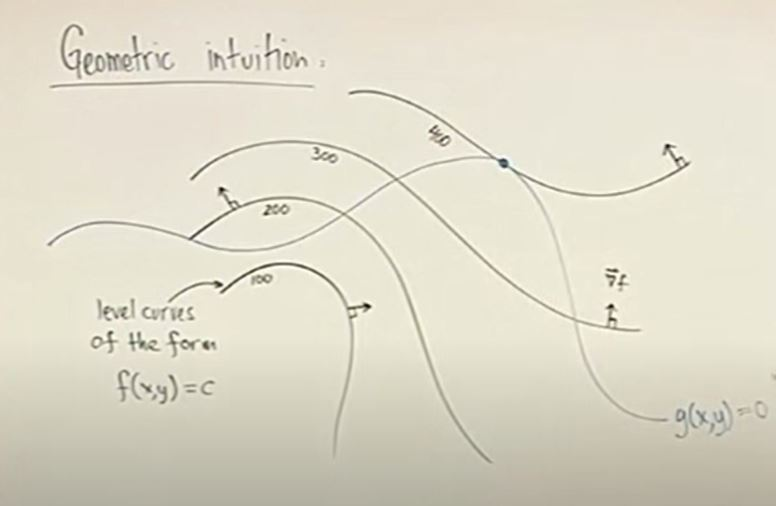
\includegraphics[scale = 0.5]{src/lagIntuition.JPG}
    \label{fig:my_label}
\end{figure}
We have limited our $x,y$ for some two variable $f$ to equal $0$. We then ask, with this constraint, at which $x,y$ does $f$ attain a maximum or a minimum. This is solved by lagrange multipliers

\begin{theorem}
Let $h,f U \to \mathbb{R}$ be of class $C^{1}$ and let $M = \{x\in U|f(x)=0\}$ Now let $a \in M$ and let $a$ be such that $h(a)$ is a local extremum. Then $\exists \lambda:$
$$\grad h(a) + \lambda \grad f(a) = 0$$

\end{theorem}


\subsection{Multiple integrals}

Define a function $$g(y) = \int_{a}^{b} f(x,y)dx$$ Now if $f$ is continuous and its partial derivatives are continuous, $f$ is $C^{1}(I)$ and we have:
$$g^{\prime}(y) = \int_{a}^{b} \frac{\partial f(x,y)}{\partial y}dx$$ Using this property, our goal is to perform integrating through differentiation. Thus we have that over a fixed finite interval, if $g$ is continuous, the integral is continuous. Similarly if $g$ is continously differentiable, then the integral is continuously differentiable. 

\begin{example}
Suppose we want to evaluate $\int_{0}^{b}x^{2}\cos{x}dx$. We define $g(y) = \int_{0}^{b}\cos{xy}dx$ Now by our above theorem we have $g^{\prime} = - \int_{0}^{b}x \sin{xy} dx$ and $g^{\prime\prime} = - \int_{0}^{b}x^{2} \cos{xy} dx$. And now $-g^{\prime\prime}(1) = \int_{0}^{b}x^{2} \cos{x} dx $ Now we may simply evaluate the integral by evaluating $g$ and differentiating twice. 
\end{example}





\end{document} 

